% !TeX spellcheck = hu_HU
% !TeX encoding = UTF-8
% !TeX program = xelatex
%----------------------------------------------------------------------------
\section{Nyelvek becsomagolása binárisba}\label{sec:ftr:dsl-pkg}
%----------------------------------------------------------------------------

Mivel a C4 nyelv nagy előnye, hogy könnyedén lehetséges benne \gls{DSL}-ek megvalósítását létrehozni, így előnyös lehet, ha az így előállított \gls{DSL}-ek akár célzottan is futtathatóvá tehetőek.
Ha például \aref{sec:uses:fsm}.~fejezetben definiált állapotgép leírást nézzük, lehetséges, hogy valakinek hasznos lenne egy külön {\tt c4fsm} bináris előállítása, amelyik előre rendelkezik az összes \gls{DSL} által igényelt definícióval, akár előre optimalizált \gls{IR} formájában beágyazva, hogy az eszköz már azonnal képes legyen értelmezni az állapotgép leírásokat.

Az architektúrában bemutatott \ref{fig:c4-comp}.~ábrán is látszik, hogy a nyelv alapjainak a feldolgozása teljesen el van különítve a végül futtatást végrehajtó egységektől.
Ezt kihasználva lehetséges megcsinálni, hogy egy olyan {\tt c4cc} (C4 Compiler Compiler) eszközt hozok létre, amelyik képes az előre \gls{IR} formára hozott \gls{DSL} leírást becsomagolni a {\tt c4i} bináris alapvető kódjába beilleszteni, és a fordítás során elérhetővé tenni ezeket.
Az így kapott rendszer komponens diagramja látható \aref{fig:c4-comp-ex}.~ábrán.

\begin{figure}[htb]
    \centerline{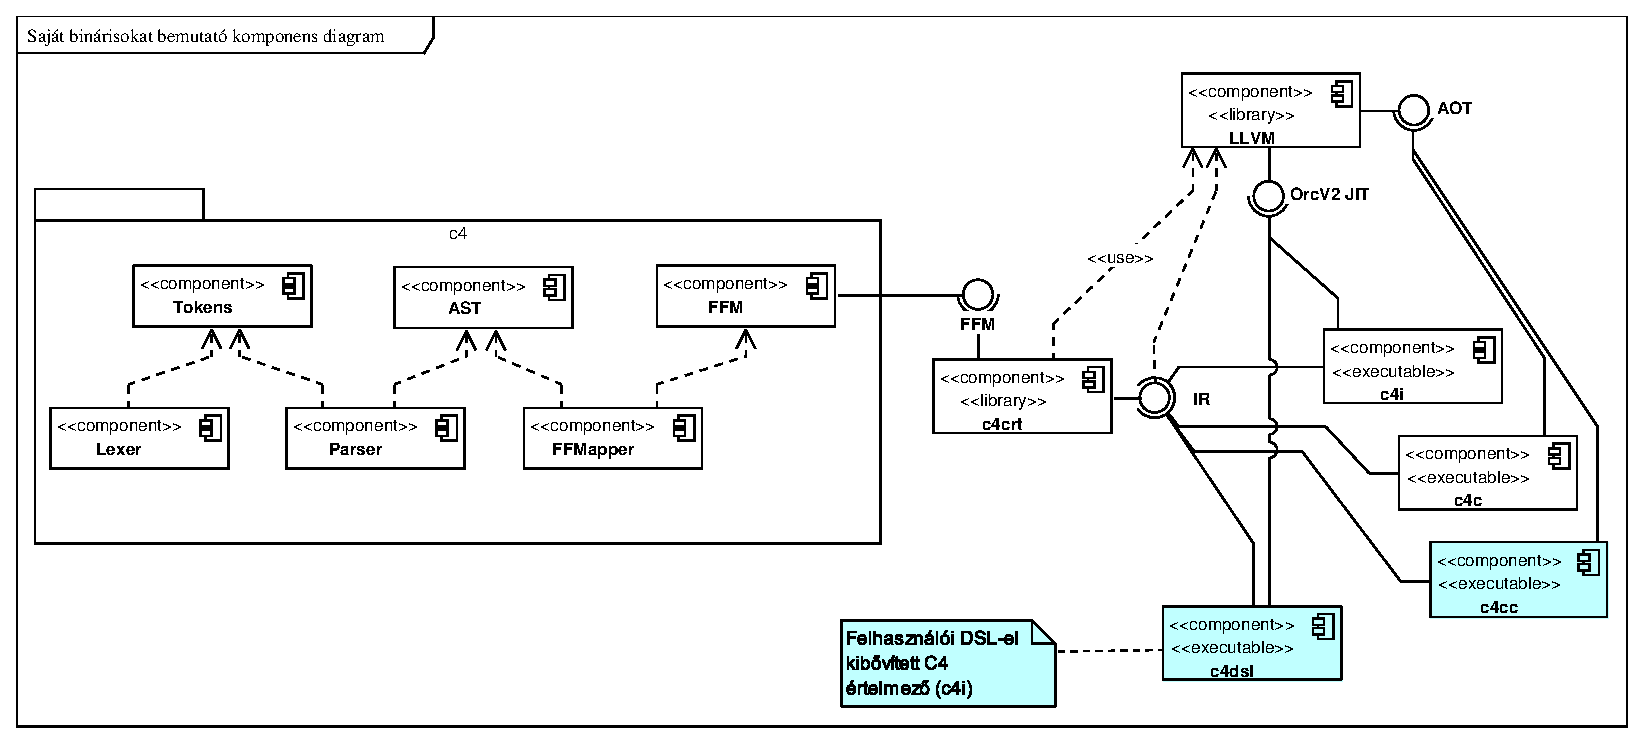
\includegraphics[width=.8\linewidth]{figures/c4-comp-ex.eps}}
    \caption{A saját bővítési lehetőségekkel ellátott komponens diagram}\label{fig:c4-comp-ex}
\end{figure}

Bár kifejezett nehézség nem származna abból, hogy a \gls{JIT} megvalósítás mellé a {\tt c4c} fordítóba is becsomagolhatóak legyenek előre megírt \gls{DSL} nyelvek, a jelenlegi használatról alkotott elképzeléseim szerint ez nem is számítana akkora előnynek.
Ilyenkor csupán a fejlesztő számára kerül telepítésre a C4 környezet, és a végfelhasználók a \gls{DSL}-ekkel leírt program viselkedésére tartanak csak igyént, míg a {\tt c4i} esetén a célközönség fejlesztők, így a \gls{DSL} számít a végterméknek.
Emiatt egyelőre nem gondolom, hogy hasonlóan érdemes lenne támogatni a {\tt c4c}-nek is a becsomagolását.
